%%%%%%%%%%%%%%%%%%%%%%%%%%%%%%%%%%%%%%%%%%%%%%%%%%%%%%%%%%%%%%%%%%%%%%%%%%%%%
% BENCHMARKING AI FACTORIES ON MELUXINA
% Final Defense Presentation - EUMaster4HPC Student Challenge 2025-2026
% Team 11
%%%%%%%%%%%%%%%%%%%%%%%%%%%%%%%%%%%%%%%%%%%%%%%%%%%%%%%%%%%%%%%%%%%%%%%%%%%%%

\documentclass[aspectratio=169,11pt]{beamer}

% --- Theme Configuration ---
\usetheme{Madrid}
\usecolortheme{whale}
\setbeamertemplate{navigation symbols}{}
\setbeamertemplate{footline}[frame number]

% --- Speaker Notes Configuration ---
\usepackage{pgfpages}
% Uncomment the following line to enable speaker notes on second screen:
%\setbeameroption{show notes on second screen=right}

% --- Packages ---
\usepackage[utf8]{inputenc}
\usepackage[T1]{fontenc}
\usepackage{graphicx}
\usepackage{booktabs}
\usepackage{tikz}
\usetikzlibrary{shapes.geometric, arrows.meta, positioning}
\usepackage{xcolor}

% --- Custom Colors ---
\definecolor{eurohpc}{RGB}{0, 82, 147}
\definecolor{accentgreen}{RGB}{46, 139, 87}
\definecolor{accentorange}{RGB}{230, 126, 34}

% --- Title Information ---
\title[AI Factory Benchmarking]{\textbf{Benchmarking AI Factories on MeluXina}}
\subtitle{A Modular Framework for Reproducible AI Workload Evaluation}
\author{Team 11}
\institute{EUMaster4HPC Student Challenge 2025-2026}
\date{January 2026}
\titlegraphic{\includegraphics[height=1.2cm]{logos/eurohpc_logo.png}\hspace{1cm}\includegraphics[height=1.2cm]{logos/meluxina_logo.png}}

\begin{document}

%%%%%%%%%%%%%%%%%%%%%%%%%%%%%%%%%%%%%%%%%%%%%%%%%%%%%%%%%%%%%%%%%%%%%%%%%%%%%
% TITLE SLIDE
%%%%%%%%%%%%%%%%%%%%%%%%%%%%%%%%%%%%%%%%%%%%%%%%%%%%%%%%%%%%%%%%%%%%%%%%%%%%%
\begin{frame}
\titlepage
\end{frame}

%%%%%%%%%%%%%%%%%%%%%%%%%%%%%%%%%%%%%%%%%%%%%%%%%%%%%%%%%%%%%%%%%%%%%%%%%%%%%
% SLIDE 1: THE PROBLEM - HOOK
%%%%%%%%%%%%%%%%%%%%%%%%%%%%%%%%%%%%%%%%%%%%%%%%%%%%%%%%%%%%%%%%%%%%%%%%%%%%%
\begin{frame}{The EUMaster4HPC Challenge}
\centering
\textbf{\large Challenge:} \textit{Benchmarking AI Factories}

\vspace{1em}
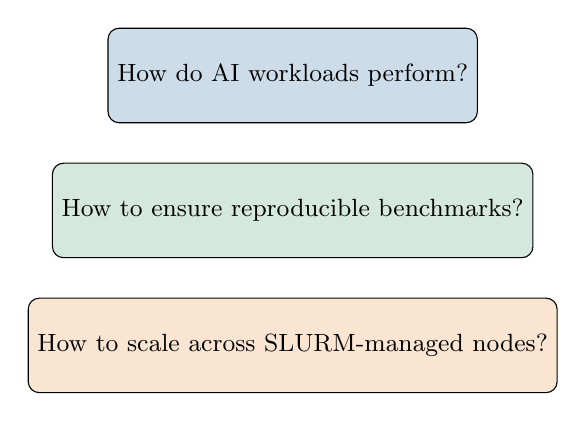
\begin{tikzpicture}[
    box/.style={rectangle, draw, rounded corners, minimum width=4.5cm, minimum height=1.2cm, font=\small, text centered}
]
\node[box, fill=eurohpc!20] (q1) {How do AI workloads perform?};
\node[box, fill=accentgreen!20, below=0.5cm of q1] (q2) {How to ensure reproducible benchmarks?};
\node[box, fill=accentorange!20, below=0.5cm of q2] (q3) {How to scale across SLURM-managed nodes?};
\end{tikzpicture}

\vspace{1em}
\textbf{Target:} vLLM inference, MinIO S3, Vector DBs on MeluXina GPU partition
\end{frame}

%%%%%%%%%%%%%%%%%%%%%%%%%%%%%%%%%%%%%%%%%%%%%%%%%%%%%%%%%%%%%%%%%%%%%%%%%%%%%
% SLIDE 2: OUR SOLUTION - HIGH LEVEL
%%%%%%%%%%%%%%%%%%%%%%%%%%%%%%%%%%%%%%%%%%%%%%%%%%%%%%%%%%%%%%%%%%%%%%%%%%%%%
\begin{frame}{Our Solution: A Modular Benchmarking Framework}
\begin{columns}
\column{0.4\textwidth}
\textbf{\large Three Pillars:}
\begin{enumerate}
    \item \textcolor{eurohpc}{\textbf{Modular}} -- 4-component design
    \item \textcolor{accentgreen}{\textbf{Reproducible}} -- YAML recipes
    \item \textcolor{accentorange}{\textbf{Scalable}} -- Native SLURM
\end{enumerate}

\vspace{1em}
\textbf{Supported Workloads:}
\begin{itemize}
    \item vLLM Inference
    \item MinIO S3 Storage
    \item (Extensible to Vector DBs)
\end{itemize}

\column{0.55\textwidth}
\centering
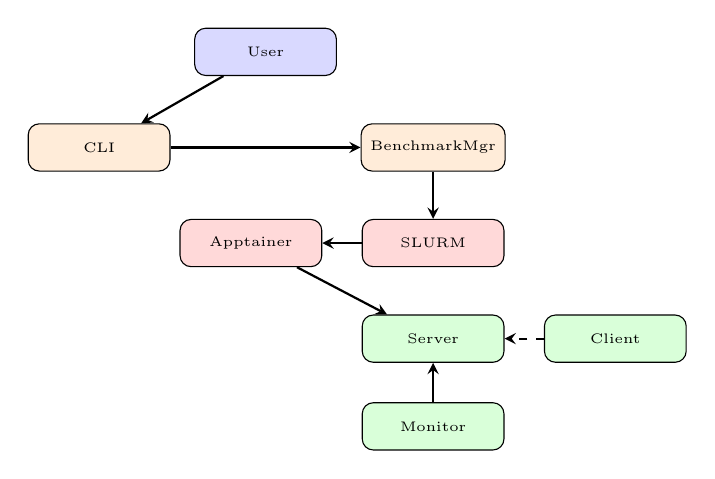
\begin{tikzpicture}[
    node distance=0.6cm and 0.8cm,
    box/.style={rectangle, draw, rounded corners, minimum width=1.8cm, minimum height=0.6cm, font=\tiny, text centered},
    userbox/.style={box, fill=blue!15},
    intbox/.style={box, fill=orange!15},
    hpcbox/.style={box, fill=red!15},
    compbox/.style={box, fill=green!15},
    arrow/.style={->, >=stealth, thick, font=\tiny}
]
\node[userbox] (user) {User};
\node[intbox, below left=0.6cm and 0.3cm of user] (cli) {CLI};
\node[intbox, below right=0.6cm and 0.3cm of user] (bm) {BenchmarkMgr};
\node[hpcbox, below=0.6cm of bm] (slurm) {SLURM};
\node[hpcbox, left=0.5cm of slurm] (appt) {Apptainer};
\node[compbox, below=0.6cm of slurm] (srv) {Server};
\node[compbox, right=0.5cm of srv] (cli2) {Client};
\node[compbox, below=0.5cm of srv] (mon) {Monitor};

\draw[arrow] (user) -- (cli);
\draw[arrow] (cli) -- (bm);
\draw[arrow] (bm) -- (slurm);
\draw[arrow] (slurm) -- (appt);
\draw[arrow] (appt) -- (srv);
\draw[arrow, dashed] (cli2) -- (srv);
\draw[arrow] (mon) -- (srv);
\end{tikzpicture}
\end{columns}
\end{frame}

%%%%%%%%%%%%%%%%%%%%%%%%%%%%%%%%%%%%%%%%%%%%%%%%%%%%%%%%%%%%%%%%%%%%%%%%%%%%%
% SLIDE 3: ARCHITECTURE DEEP DIVE
%%%%%%%%%%%%%%%%%%%%%%%%%%%%%%%%%%%%%%%%%%%%%%%%%%%%%%%%%%%%%%%%%%%%%%%%%%%%%
\begin{frame}{System Architecture: Four-Module Design}
\centering
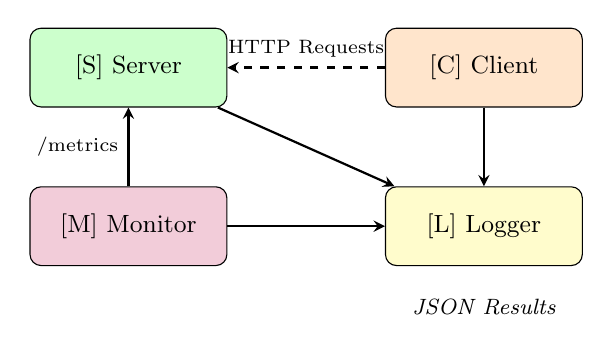
\begin{tikzpicture}[
    node distance=1cm and 1.5cm,
    box/.style={rectangle, draw, rounded corners, minimum width=2.5cm, minimum height=1cm, font=\small, text centered},
    serverbox/.style={box, fill=green!20},
    clientbox/.style={box, fill=orange!20},
    monitorbox/.style={box, fill=purple!20},
    loggerbox/.style={box, fill=yellow!20},
    arrow/.style={->, >=stealth, thick}
]

\node[serverbox] (server) {[S] Server};
\node[clientbox, right=2cm of server] (client) {[C] Client};
\node[monitorbox, below=1cm of server] (monitor) {[M] Monitor};
\node[loggerbox, below=1cm of client] (logger) {[L] Logger};

\draw[arrow, dashed] (client) -- node[above, font=\scriptsize] {HTTP Requests} (server);
\draw[arrow] (monitor) -- node[left, font=\scriptsize] {/metrics} (server);
\draw[arrow] (server) -- (logger);
\draw[arrow] (client) -- (logger);
\draw[arrow] (monitor) -- (logger);

\node[below=0.3cm of logger, font=\footnotesize\itshape] {JSON Results};

\end{tikzpicture}

\vspace{0.5em}
\begin{tabular}{cccc}
\textcolor{green!50!black}{\textbf{Server}} & \textcolor{orange!70!black}{\textbf{Client}} & \textcolor{purple!70!black}{\textbf{Monitor}} & \textcolor{yellow!50!black}{\textbf{Logger}} \\
vLLM, MinIO & Load Generator & Prometheus Scraper & Thread-safe JSON
\end{tabular}
\end{frame}

%%%%%%%%%%%%%%%%%%%%%%%%%%%%%%%%%%%%%%%%%%%%%%%%%%%%%%%%%%%%%%%%%%%%%%%%%%%%%
% SLIDE 4: EXECUTION FLOW
%%%%%%%%%%%%%%%%%%%%%%%%%%%%%%%%%%%%%%%%%%%%%%%%%%%%%%%%%%%%%%%%%%%%%%%%%%%%%
\begin{frame}{Execution Flow: From Recipe to Results}
\vfill
\centering
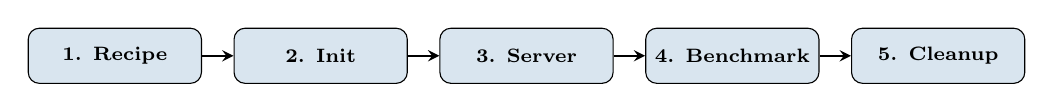
\begin{tikzpicture}[
    phase/.style={rectangle, draw, rounded corners, fill=eurohpc!15, minimum width=2.2cm, minimum height=0.7cm, font=\scriptsize\bfseries},
    arrow/.style={->, >=stealth, thick}
]
\node[phase] (p1) {1. Recipe};
\node[phase, right=0.4cm of p1] (p2) {2. Init};
\node[phase, right=0.4cm of p2] (p3) {3. Server};
\node[phase, right=0.4cm of p3] (p4) {4. Benchmark};
\node[phase, right=0.4cm of p4] (p5) {5. Cleanup};

\draw[arrow] (p1) -- (p2);
\draw[arrow] (p2) -- (p3);
\draw[arrow] (p3) -- (p4);
\draw[arrow] (p4) -- (p5);
\end{tikzpicture}
\vfill
\end{frame}

%%%%%%%%%%%%%%%%%%%%%%%%%%%%%%%%%%%%%%%%%%%%%%%%%%%%%%%%%%%%%%%%%%%%%%%%%%%%%
% SLIDE 5: REPRODUCIBILITY - YAML RECIPES
%%%%%%%%%%%%%%%%%%%%%%%%%%%%%%%%%%%%%%%%%%%%%%%%%%%%%%%%%%%%%%%%%%%%%%%%%%%%%
\begin{frame}{Reproducibility: Declarative YAML Recipes}
\begin{columns}
\column{0.5\textwidth}
\textbf{\large Recipe = Complete Experiment}
\begin{itemize}
    \item Model, container image
    \item Resource allocation
    \item Client concurrency
    \item Monitoring targets
    \item Cleanup actions
\end{itemize}

\vspace{0.5em}
\textcolor{accentgreen}{$\checkmark$} \textbf{Git-versioned, shareable}

\column{0.5\textwidth}
\footnotesize
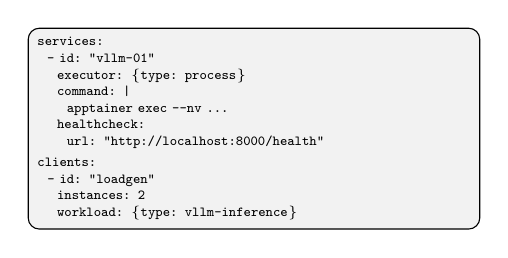
\begin{tikzpicture}
\node[draw, fill=gray!10, rounded corners, text width=5.5cm, font=\ttfamily\tiny, align=left] {
services:\\
\ \ - id: "vllm-01"\\
\ \ \ \ executor: \{type: process\}\\
\ \ \ \ command: |\\
\ \ \ \ \ \ apptainer exec --nv ...\\
\ \ \ \ healthcheck:\\
\ \ \ \ \ \ url: "http://localhost:8000/health"\\[0.3em]
clients:\\
\ \ - id: "loadgen"\\
\ \ \ \ instances: 2\\
\ \ \ \ workload: \{type: vllm-inference\}
};
\end{tikzpicture}
\end{columns}
\end{frame}

%%%%%%%%%%%%%%%%%%%%%%%%%%%%%%%%%%%%%%%%%%%%%%%%%%%%%%%%%%%%%%%%%%%%%%%%%%%%%
% SLIDE 7: RESULTS OVERVIEW
%%%%%%%%%%%%%%%%%%%%%%%%%%%%%%%%%%%%%%%%%%%%%%%%%%%%%%%%%%%%%%%%%%%%%%%%%%%%%
\begin{frame}{Experimental Results: MeluXina GPU Partition}
\centering
\begin{table}
\scriptsize
\begin{tabular}{lcc}
\toprule
\textbf{Metric} & \textbf{vLLM Inference} & \textbf{MinIO S3} \\
\midrule
Duration & 120s & 300s \\
Clients & 2 instances $\times$ 4 threads & 4 instances $\times$ 4 threads \\
Model/Target & facebook/opt-125m & Object PUT/GET \\
\midrule
\textbf{Total Ops} & 3,680 requests & $\sim$6,800 objects \\
\textbf{Throughput} & 15.2 req/s (per client) & 145 MB/s (per client) \\
\textbf{Latency Avg} & 125.5 ms & PUT: 530ms / GET: 360ms \\
\textbf{Latency P95} & 195.7 ms & PUT: 960ms / GET: 670ms \\
\textbf{Tokens/s} & 1,437 tokens/s & -- \\
\textbf{Success Rate} & 99.9\% & 100\% \\
\bottomrule
\end{tabular}
\end{table}
\end{frame}

%%%%%%%%%%%%%%%%%%%%%%%%%%%%%%%%%%%%%%%%%%%%%%%%%%%%%%%%%%%%%%%%%%%%%%%%%%%%%
% SLIDE 8: vLLM RESULTS - GRAFANA
%%%%%%%%%%%%%%%%%%%%%%%%%%%%%%%%%%%%%%%%%%%%%%%%%%%%%%%%%%%%%%%%%%%%%%%%%%%%%
\begin{frame}{vLLM Inference: Real-Time Metrics}
\centering
\includegraphics[width=0.95\textwidth]{diagrams/grafana_vllm.png}

\vspace{0.3em}
\small Panel 1: Request Rate | Panel 2: Concurrent Requests | Panel 3: Latency Heatmap
\end{frame}

%%%%%%%%%%%%%%%%%%%%%%%%%%%%%%%%%%%%%%%%%%%%%%%%%%%%%%%%%%%%%%%%%%%%%%%%%%%%%
% SLIDE 9: S3 RESULTS - GRAFANA
%%%%%%%%%%%%%%%%%%%%%%%%%%%%%%%%%%%%%%%%%%%%%%%%%%%%%%%%%%%%%%%%%%%%%%%%%%%%%
\begin{frame}{MinIO S3: Object Storage Performance}
\centering
\includegraphics[width=0.95\textwidth]{diagrams/grafana_s3.png}

\vspace{0.3em}
\begin{columns}
\column{0.33\textwidth}
\centering
\textbf{Panel 1}\\Total Requests\\(per client)
\column{0.33\textwidth}
\centering
\textbf{Panel 2}\\Traffic Sent\\(400-700 MB bursts)
\column{0.33\textwidth}
\centering
\textbf{Panel 3}\\TTFB Heatmap\\(latency buckets)
\end{columns}
\end{frame}

%%%%%%%%%%%%%%%%%%%%%%%%%%%%%%%%%%%%%%%%%%%%%%%%%%%%%%%%%%%%%%%%%%%%%%%%%%%%%
% SLIDE 10: VISUALIZATION INFRASTRUCTURE
%%%%%%%%%%%%%%%%%%%%%%%%%%%%%%%%%%%%%%%%%%%%%%%%%%%%%%%%%%%%%%%%%%%%%%%%%%%%%
\begin{frame}{Built-in Visualization: FastAPI + Grafana}
\begin{columns}
\column{0.5\textwidth}
\textbf{\large FastAPI Server Features:}
\begin{itemize}
    \item Grafana SimpleJSON datasource
    \item Auto-detects service type
    \item Applies \texttt{rate()} to counters
    \item Zero external dependencies
\end{itemize}

\vspace{0.5em}
\textbf{\large Usage:}\\
\texttt{python fastapi\_server.py}\\
$\rightarrow$ Connect Grafana to \texttt{localhost:8000}

\column{0.5\textwidth}
\centering
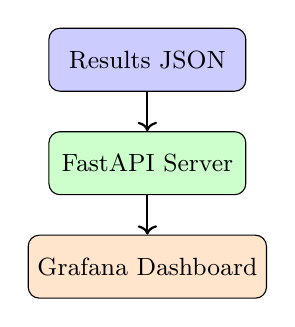
\begin{tikzpicture}[
    box/.style={rectangle, draw, rounded corners, minimum width=2.5cm, minimum height=0.8cm, font=\small}
]
\node[box, fill=blue!20] (results) {Results JSON};
\node[box, fill=green!20, below=0.5cm of results] (fastapi) {FastAPI Server};
\node[box, fill=orange!20, below=0.5cm of fastapi] (grafana) {Grafana Dashboard};

\draw[->, thick] (results) -- (fastapi);
\draw[->, thick] (fastapi) -- (grafana);
\end{tikzpicture}
\end{columns}
\end{frame}

%%%%%%%%%%%%%%%%%%%%%%%%%%%%%%%%%%%%%%%%%%%%%%%%%%%%%%%%%%%%%%%%%%%%%%%%%%%%%
% SLIDE 11: EXTENSIBILITY
%%%%%%%%%%%%%%%%%%%%%%%%%%%%%%%%%%%%%%%%%%%%%%%%%%%%%%%%%%%%%%%%%%%%%%%%%%%%%
\begin{frame}{Extensibility: Adding New Workloads}
\centering
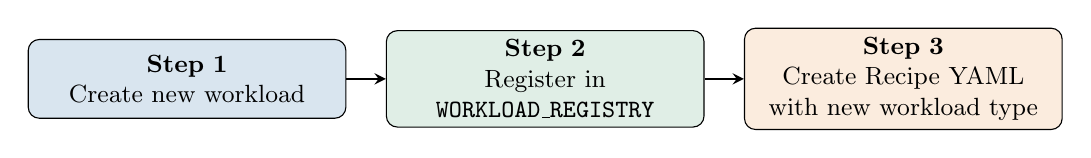
\begin{tikzpicture}[
    box/.style={rectangle, draw, rounded corners, minimum width=4cm, minimum height=1cm, font=\small, text centered, text width=3.8cm},
    arrow/.style={->, >=stealth, thick}
]

\node[box, fill=eurohpc!15] (step1) {\textbf{Step 1}\\Create new workload};
\node[box, fill=accentgreen!15, right=0.5cm of step1] (step2) {\textbf{Step 2}\\Register in\\\texttt{WORKLOAD\_REGISTRY}};
\node[box, fill=accentorange!15, right=0.5cm of step2] (step3) {\textbf{Step 3}\\Create Recipe YAML\\with new workload type};

\draw[arrow] (step1) -- (step2);
\draw[arrow] (step2) -- (step3);

\end{tikzpicture}

\end{frame}

%%%%%%%%%%%%%%%%%%%%%%%%%%%%%%%%%%%%%%%%%%%%%%%%%%%%%%%%%%%%%%%%%%%%%%%%%%%%%
% SLIDE 12: CONCLUSION
%%%%%%%%%%%%%%%%%%%%%%%%%%%%%%%%%%%%%%%%%%%%%%%%%%%%%%%%%%%%%%%%%%%%%%%%%%%%%
\begin{frame}{Conclusion: Key Takeaways}
\centering
\textbf{\large What We Delivered:}

\vspace{0.8em}
\begin{columns}
\column{0.33\textwidth}
\centering

\begin{tikzpicture}
\node[draw, fill=eurohpc!20, rounded corners, minimum width=2.5cm, minimum height=1.5cm] {\textbf{HPC-Native}};
\end{tikzpicture}\\[0.3em]
\footnotesize SLURM + Apptainer integration
\column{0.33\textwidth}
\centering
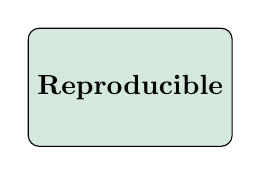
\begin{tikzpicture}
\node[draw, fill=accentgreen!20, rounded corners, minimum width=2.5cm, minimum height=1.5cm] {\textbf{Reproducible}};
\end{tikzpicture}\\[0.3em]
\footnotesize YAML Recipe files
\column{0.33\textwidth}
\centering
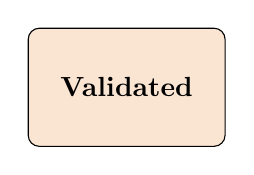
\begin{tikzpicture}
\node[draw, fill=accentorange!20, rounded corners, minimum width=2.5cm, minimum height=1.5cm] {\textbf{Validated}};
\end{tikzpicture}\\[0.3em]
\footnotesize validated on MeluXina
\end{columns}

\vspace{1.2em}
\textbf{Impact:} Enables EuroHPC users to scientifically benchmark\\AI Factory components with minimal setup.

\vspace{1.5em}
\Large \textbf{Questions?}
\end{frame}

%%%%%%%%%%%%%%%%%%%%%%%%%%%%%%%%%%%%%%%%%%%%%%%%%%%%%%%%%%%%%%%%%%%%%%%%%%%%%
% BACKUP SLIDES
%%%%%%%%%%%%%%%%%%%%%%%%%%%%%%%%%%%%%%%%%%%%%%%%%%%%%%%%%%%%%%%%%%%%%%%%%%%%%
\appendix

\begin{frame}{Backup: Technology Stack}
\begin{table}
\begin{tabular}{ll}
\toprule
\textbf{Component} & \textbf{Technology} \\
\midrule
Language & Python 3.9+ \\
Configuration & PyYAML \\
HTTP & requests, FastAPI \\
Metrics & Prometheus format, matplotlib \\
Containers & Apptainer/Singularity \\
Scheduler & SLURM \\
Visualization & Grafana SimpleJSON \\
\bottomrule
\end{tabular}
\end{table}
\end{frame}

\begin{frame}{Backup: Error Handling}
\textbf{Multi-level Resilience:}
\begin{itemize}
    \item Healthcheck timeout $\rightarrow$ graceful shutdown
    \item Executor stop isolation $\rightarrow$ prevents cascading failures
    \item Workload error backoff $\rightarrow$ configurable retry with abort threshold
    \item Monitor resilience $\rightarrow$ continues on scrape failures
\end{itemize}
\end{frame}

\end{document}
